\textbf{Цель работы:} исследовать свойства постоянных неодимовых магнитов; измерить с их помощью горизонтальную и вертикальную составляющие индукции магнитного поля Земли и магнитное наклонение. \\

\textbf{Используемое оборудование:} неодимовые магниты; тонкая нить для изготовления крутильного маятника; медная проволока; электронные весы; секундомер; измеритель магнитной индукции; штангенциркуль; брусок, линейка и штатив из немагнитных материалов; набор гирь и разновесов. 
                    
\section{Теоретическое введение}

Магнитное поле точечного диполя с магнитным моментом $\textbf{m} = \textbf{S}I$ определяется по формуле, аналогичной формуле для поля элементарного электрического диполя:

\begin{equation}
    \textbf{B}_{\text{дип}} = \frac{\mu_0}{4 \pi} \left( \frac{3(\textbf{m} \cdot \textbf{r})\textbf{r}}{r^5} - \frac{\textbf{m}}{r^3}  \right)
\end{equation}

При этом сила, действующая на диполь, равна 

\begin{equation}
    \textbf{F} = (\textbf{m} \cdot \triangledown ) \textbf{B}
\end{equation}

А момент силы равен

\begin{equation}
    \textbf{M} = [ \textbf{m} \times \textbf{B}] 
\end{equation}

В частном случае, когда моменты двух небольших магнитов направлены вдоль соединяющей их прямой, сила их взаимодействия равна

\begin{equation}
    F = - \frac{6 m_1 m_2}{r^4}
\end{equation}

Если магнитные моменты направлены перпендикулярно соединяющей их прямой, то

\begin{equation}
    F = \frac{3 m_1 m_2}{r^4}
\end{equation}

\section{Экспериментальное оборудование и методика измерений}

\subsection{Определение магнитного момента магнитных шариков}

\subsubsection{Метод 1}

Величину магнитного момента $m$ двух одинаковых шариков можно рассчитать, зная их массу $M$ и определив максимальное расстояние $r_{max}$, на котором они ещё удерживают друг друга в поле тяжести (см. рис.). Из формулы для взаимодействия диполей имеем

\begin{equation}
    m = \sqrt{\frac{Mgr^4_{max}}{6}}
\end{equation}

Таким образом с помощью измеренного магнитного момента шарика можно измерить индукцию магнитного поля

\begin{figure}[h]
    \centering
    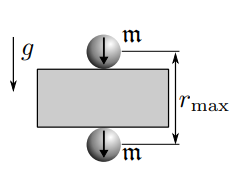
\includegraphics[width = 5 cm]{images/1.png}
    \caption{Измерение магнитных моментов шариков}
    \label{msh1}
\end{figure}

\subsubsection{Метод 2}

Величину магнитного момента шариков можно определить также по силе их сцепления. Она определяется как сила, необходимая для разрыва двух сцепившихся магнитных шариков. Сила сцепления максимальна, если шары соединяются своими противоположными полюсами (магнитные моменты сонаправлены). 

Максимальную силу сцепления можно определить по весу магнитной цепочки, которую способен удержать самый верхний магнитный шарик. При этом для расчёта прочности цепочки достаточно учитывать силу взаимодействия верхнего шара с 3–4 ближайшими соседями.

\begin{equation}
    F = \frac{3m^2}{8R^4} \left( 1 + \frac{1}{2^4} + \frac{1}{3^4} + ...\right) = 1,08 \cdot \frac{3m^2}{8R^4}
\end{equation}

\subsection{Измерение горизонтальной составляющей индукции магнитного поля Земли}

Магнитное поле Земли можно измерить по периоду крутильных колебаний «магнитной стрелки» вокруг вертикальной оси. 

«Магнитная стрелка» образована сцепленными друг с другом $n$ намагниченными шариками. Для крепления нити в работе используется штатив, изготовленный из немагнитного материала. Магнитные моменты всех шариков направлены в одну сторону вдоль оси «стрелки». При отклонении стрелки на угол $\theta$ от равновесного положения в горизонтальной плоскости возникают крутильные колебания вокруг вертикальной оси, проходящей через середину стрелки.

\begin{figure}[h]
    \centering
    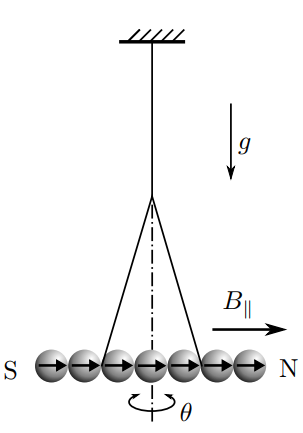
\includegraphics[width = 6 cm]{images/2.png}
    \caption{ Крутильный маятник во внешнем магнитном поле}
    \label{sh1}
\end{figure}

\begin{equation}
    M = -m_n B_{||} \sin{\theta} \Rightarrow J_n \ddot{\theta} + m_n B_{||} \theta = 0 \Rightarrow T = 2 \pi \sqrt{\frac{J_n}{m_n B_{||}}}
\end{equation}

\begin{equation}
    T = 2 \pi \sqrt{\frac{J_n}{m_n B_{||}}} = 2 \pi \sqrt{\frac{n^3 M R^2}{12m_n B_{||}}} \Rightarrow T = 2 \pi \sqrt{\frac{M R^2}{3 m B_{||}}} n
\end{equation}

\subsection{Измерение вертикальной составляющей индукции магнитного поля Земли. Магнитное наклонение}

Для измерения вертикальной составляющей вектора индукции поля Земли используется та же установка, что и для измерения горизонтальной составляющей с тем лишь отличием, что подвешенная магнитная «стрелка» закрепляется на нити в одной точке. В этом случае стрелка, составленная из чётного числа одинаковых шариков и подвешенная за середину, расположится не горизонтально, а под некоторым углом к горизонту.

Это связано с тем, что вектор $\textbf{B}$ индукции магнитного поля Земли не горизонтален, а образует с горизонтом
некоторый угол $\beta$, зависящий от географической широты $\phi$ места, где проводится опыт. Величина угла $\beta$ называется магнитным наклонением.

\begin{figure}[h]
    \centering
    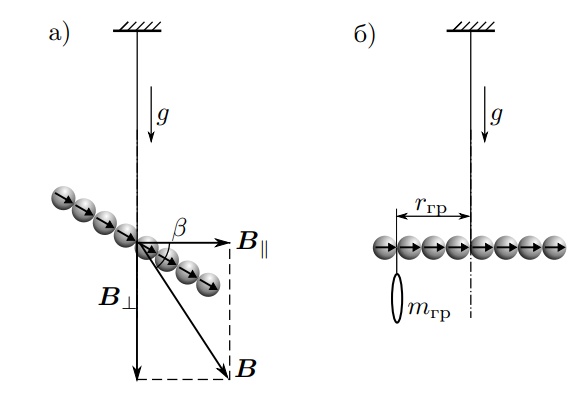
\includegraphics[width = 10 cm]{images/3.png}
    \caption{Измерение вертикальной составляющей поля и магнитного наклонения}
    \label{way3}
\end{figure}

\begin{equation}
    M_n = m B_{\perp} n
\end{equation}

\section{Ход работы}

\subsection{Измерение магнитного момента шарика}

\subsubsection{Метод 1}

Диаметр используемых шариков равен $D = 5,908 \pm 0,008$, масса $M = 0,8422 \pm 0,0002$ г. Откуда имеем для радиуса величину $R = 2,954 \pm 0,004$.

С помощью магнетометра измерим индукцию магнитного поля на полюсах системы из двух шариков $B_{p2} = 304 \pm 1$ мТл, откуда, с учётом поправок на поле второго шарика в виде $\left( \frac{1}{3} \right)^3 = 0,037$, имеем $B_{p} = 293 \pm 1$ мТл.

Между двумя магнитными шариками разместим брусок из немагнитного материала. Подкладывая между бруском и верхним магнитиком листы бумаги, определим, на каком максимальном расстоянии шарики удерживают друг друга в поле тяжести Земли: $r_{max} = 1,47 \pm 0,01$ см, откуда находим

\begin{equation}
    m = \sqrt{\frac{Mgr^4_{max}}{6}} = 25,341 \pm 0,017 \; \text{эрг}/\text{Гс}
\end{equation}

Погрешность магнитного момента учитывает погрешности массы и величины $r_{max}$. 

\subsubsection{Метод 2}

Используя дополнительные шарики, составим цепочку из $12$ шариков, и с помощью неодимовых магнитов в форме параллелепипедов, подсоединим цепочку к гире и разновесам так, чтобы вес системы цепочки с гирей, при котором она отрывается от верхнего шарика, был минимален: $M_{\text{оторв}} = 327 \pm 10$ г (погрешность возникает из-за методики измерений, так как измерение массы ограничивается подвешиванием фиксированного количества грузиков фиксированной массы).

\begin{equation}
    F = 1,08 \cdot \frac{3m^2}{8R^4} = M_{\text{оторв}} g \Rightarrow m = \sqrt{ \frac{8 M_{\text{оторв}} R^4 g}{3,24} }
\end{equation}

Отсюда посчитаем значение магнитного момента:

\begin{equation}
    m = 77,623 \pm 0,019 \; \text{эрг}/\text{Гс}
\end{equation}

\subsubsection{Рассчёт остаточной намагниченности}

Рассчитаем величину остаточной индукции шариков, используя результаты из двух различных методов:

Метод 1:

\begin{equation}
    B_{r1} = 4 \pi M = 4 \pi \frac{3m}{4 \pi R^3} = \frac{3m}{R^3} = 2991 \pm 6 \; \text{Гс}
\end{equation}

Метод 2:

\begin{equation}
    B_{r2} = \frac{3m}{R^3} = 9162 \pm 7 \; \text{Гс}
\end{equation}

Теоретическое же значение составляет $B_r = 12,2$ кГс.

Измерим теперь величину остаточной намагниченности экспериментальным путём, через значение магнитной индукции на полюсе шарика, которые было подсчитано ранее.

\begin{equation}
    B_r = \frac{3}{2} B_p = 4395 \pm 15 \; \text{Гс}
\end{equation}

Как можно наблюдать, даже при многократных измерениях значения, полученные тремя разными путями, расходятся довольно сильно.

Для дальнейших расчётов будем использовать значение остаточной индукции, полученное магнетометром, так как этот способ обладает наименьшей косвенностью определения этой величины. Для этого случая имеем магнитный момент шарика $37,23 \pm 0,02 \; \text{эрг}/\text{Гс}$.

\subsection{Определение горизонтальной составляющей магнитного поля Земли}

Для начала рассмотрим, как упругость нити, на которой будут подвешены магниты, влияет на период колебаний системы. Собрав окружность из шариков, тем самым сделав их магнитный момент равным нулю, подвесим её в нити и возбудим систему. Даже при минимально возможных возбуждениях возвращающей силы упругости нити не хватает, значит ей и вовсе можно пренебречь.

Соберём стрелку из шариков в количестве $n$ штук, подвесим её к нити и исследуем период колебаний системы от количества шариков $n$:

\begin{table}[h!]
    \centering
    \begin{tabular}{|c|c|c|c|c|c|}
    \hline
    \cellcolor[HTML]{FFFFFF}{\color[HTML]{000000} \textbf{$T$, с}} & \multicolumn{1}{r|}{0,724} & \multicolumn{1}{r|}{0,975} & \multicolumn{1}{r|}{1,174} & \multicolumn{1}{r|}{1,423} & \multicolumn{1}{r|}{1,681} \\ \hline
    \textbf{n}                                                     & 3                          & 4                          & 5                          & 6                          & 7                          \\ \hline
    \cellcolor[HTML]{FFFFFF}\textbf{$T$, с}                        & \multicolumn{1}{r|}{1,935} & \multicolumn{1}{r|}{2,189} & \multicolumn{1}{r|}{2,441} & \multicolumn{1}{r|}{2,652} & \multicolumn{1}{r|}{2,901} \\ \hline
    \textbf{n}                                                     & 8                          & 9                          & 10                         & 11                         & 12                         \\ \hline
    \end{tabular}
\end{table}

Построим график зависимости:

\begin{figure}[h]
    \centering
    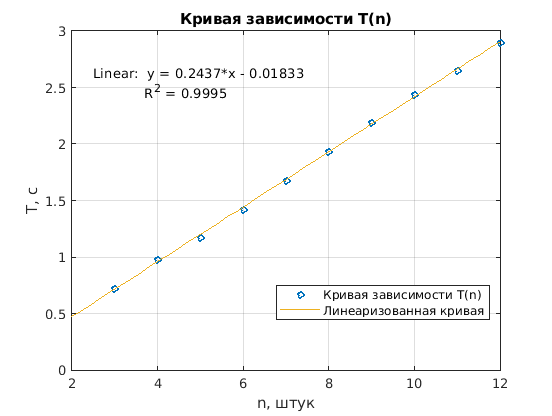
\includegraphics[width = 10 cm]{images/tn.png}
    \caption{График зависимости $T(n)$}
    \label{tn}
\end{figure}

Методом наименьших квадратов (МНК) посчитаем коэффициент наклона прямой: 

\begin{equation}
    k = 2 \pi \sqrt{\frac{M R^2}{3 m B_{||}}} = 0,2437 \pm 0,0092 \; \text{с}^{-1}
\end{equation}

\begin{equation}
    B_{||} = 201 \pm 14 \; \text{мГс}
\end{equation}

\subsection{Определение вертикальной составляющей магнитного поля Земли}

Подвесим теперь стрелку из магнитных шариков с чётным $n$ и, пользуясь ранее описанной схемой, измерим моменты сил такие, чтобы стрелка приняла горизонтальный вид:

\begin{table}[h!]
    \centering
    \begin{tabular}{|c|c|c|c|c|c|}
    \hline
    \textbf{$M$, дин $\cdot$ см} & 59,50 & 101,80 & 138,32 & 167,70 & 194,47 \\ \hline
    \textbf{n}                   & 4     & 6      & 8      & 10     & 12     \\ \hline
    \end{tabular}
\end{table}

Построим график этой зависимости ($M(n)$):

\begin{figure}[h!]
    \centering
    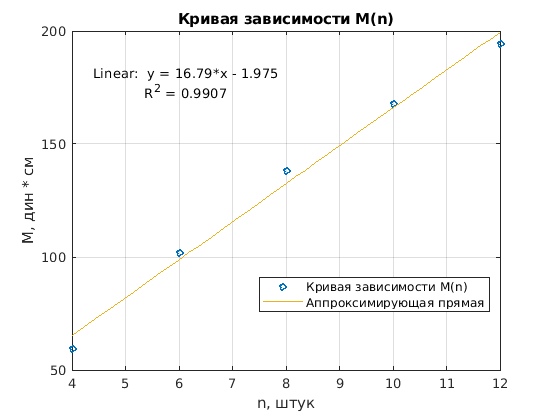
\includegraphics[width = 10 cm]{images/mn.png}
    \caption{График зависимости $M(n)$}
    \label{mn}
\end{figure}

Из МНК имеем $m B_{\perp} = 16,76 \pm 0,41 \; \text{дин} \cdot \text{см}$, откуда $B_{\perp} = 453 \pm 21$ мГс.

Тогда наклонный угол равен $arctg(\frac{B_{\perp}}{B_{||}}) \cong (66 \pm 3)^{o}$, а абсолютная величина поля равна $B = \sqrt{B_{\perp}^2 + B_{||}^2} = 495 \pm 25$ мГс.

\section{Заключение}

Несмотря на неточность методов, в частности больших расхождений в результатах измерений разными способами дипольного момента шарика, величина наклонного угла получилась практически совпадающей с табличными значениями ($\cong 70^o$), а величина индукции магнитного поля по порядку совпадает с действительной величиной ($B \cong 250$ Гс).



























